\documentclass[UTF8]{ctexart}
\usepackage{amsmath,graphicx,tikz,caption,subfigure}
\usepackage[algo2e,ruled,vlined]{algorithm2e}
\usepackage{stfloats}
\usepackage{float}
\usepackage[a4paper]{geometry}
\geometry{left=0.5cm,right=0.5cm,top=0.5cm,bottom=0.5cm}
\title{\textbf{Report1}}
\author{胡琦浩  PB21000235}
\date{\today}

\begin{document}
\maketitle

\section{问题}
用Schrage方法编写随机数子程序,用指定间隔(非连续 $l >1$)
两个随机数作为点的坐标值绘出若干点的平面分布图。再用
$<x_k>$测试均匀性(取不同量级的N值,讨论偏差与N的关系)、
$C(l)$ 测试其2维独立性(总点数$N > 10^7$)

\section{关于代码一点说明}
\begin{figure}[htbp]
    \centering
    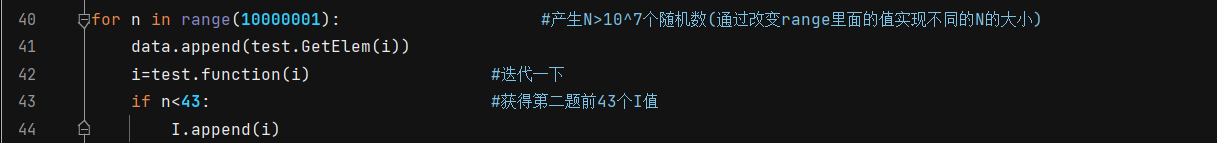
\includegraphics[scale=0.5]{2}
    \caption{main.py中的源代码片段}
\end{figure}
如图所示,由于我编写的程序中N的值需要手动修改。在测试k阶矩和卡方分布时,我将N的值依次设为$10^7+1$,$10^6+1$,$10^5+1$,得到了此实验报告的数据。但最后我将原代码中的N值又改回了$10^7+1$并生成了可执行文件,由于时间的差异导致初始值的不同,我的可执行文件中所展示$N=10^7+1$时的数据与此报告中的数据略有差异,但并不影响此报告结论的得出。

此外,由于最后程序设置的$N=10^7+1$比较大,执行程序输出结果大概要1分钟左右。

\section{方法}
用16807产生器产生随机数
\begin{equation}
    I_{n+1}=(aI_n+b)mod \quad m
\end{equation}
\begin{equation}
    x_n=I_n/m
\end{equation}

我们取$a=7^5=16807$,\quad $b=0$,\quad$m=2^{31}-1=2147483647$

考虑到$aI_n$可能越界,故采用Schrage方法:
\[
    I_{n+1} =
\begin{cases}
    a(I_nmod m)-r[I_n/q]  & I_{n+1}\mbox{>= 0} \\
    a(I_n mod  m)-r[I_n/q]+m & I_{n+1}\mbox{<0}
\end{cases}
\]

式中:$q=127773$,\quad$r=2836$

在代码实现中,利用递推算法依次得到$I_n$与$x_n$

初始$I_0$由计算机中的时间获得:
\begin{equation}
    I_0=i_y+70(i_m+12(i_d+31(i_h+23(i_n+59i_s))))
\end{equation}

\section{实验结果}
\subsection{随机数的平面分布图}
\begin{figure}[htbp]
    \centering
    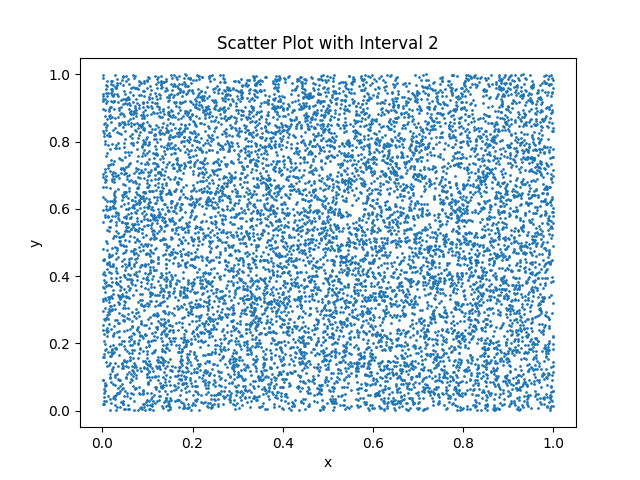
\includegraphics[scale=0.5]{figure.png}
    \caption{随机数分布图}
\end{figure}
此图中取了10000个点作图,间隔为2.由图可以看出无明显的分层现象,故随机数之间无较强的相关性

\subsection{检验随机数均匀性}
\subsubsection{利用k阶矩检验}
\begin{equation}
    <x^k>=\frac{1}{N}\sum_{i = 1}^{N} x_i^k \Rightarrow \int_{0}^{1} x^kp(x) \,dx =\frac{1}{k+1}
\end{equation}
则:
\begin{equation}
    \left\lvert <x^k>-\frac{1}{k+1}\right\rvert\approx O(\frac{1}{\sqrt{N} }) 
\end{equation}
\begin{figure}[htbp]
    \centering
    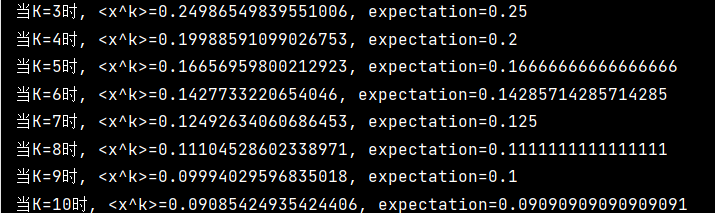
\includegraphics[scale=0.5]{10^7频率.png}
    \caption{$N=10^7+1$}
\end{figure}
\begin{figure}[htbp]
    \centering
    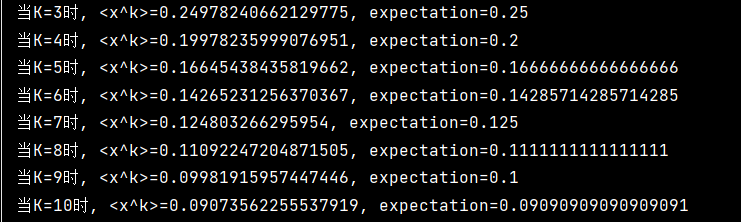
\includegraphics[scale=0.5]{10^6频率.png}
    \caption{$N=10^6+1$}
\end{figure}
\begin{figure}[htbp]
    \centering
    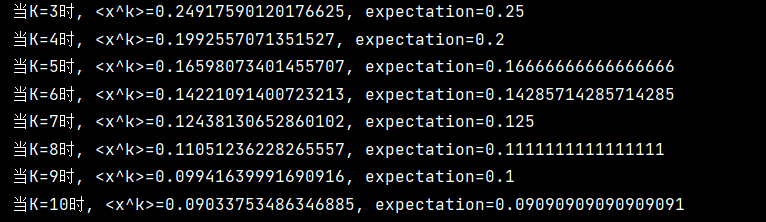
\includegraphics[scale=0.5]{10^5频率.png}
    \caption{$N=10^5+1$}
\end{figure}

不难看出,随着N的值越来越大,$<x^k>$的值与理论值越来越接近.当然,极其接近理论值的$<x^k>$表明由Schrage得到的随机数均匀性很好
\subsubsection{利用卡方检验}
将区间[0,1]分为$K$个子区间,统计随机数落在第$k $个子区间的实际频数$n_k$,它应当趋近于理论频数$m_k=\frac{N}{K}$,($k=1,2,...,K$)
令统计量:
\begin{equation}
    \chi ^2=\sum_{k = 1}^{K}  \frac{(n_k-m_k)^2}{m_k}
\end{equation}

服从自由度为$K-1$的卡方分布
\begin{figure}[H]
    \centering
    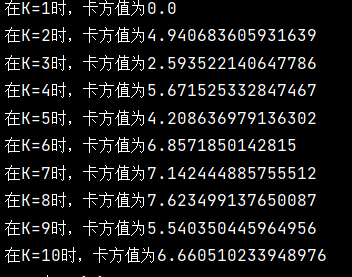
\includegraphics[scale=0.5]{10^7卡方.png}
    \caption{$N=10^7+1$}
\end{figure}
\begin{figure}[H]
    \centering
    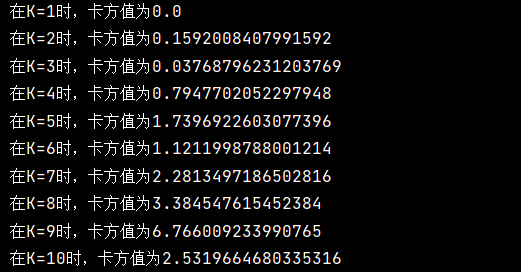
\includegraphics[scale=0.5]{10^6卡方.png}
    \caption{$N=10^6+1$}
\end{figure}
\begin{figure}[H]
    \centering
    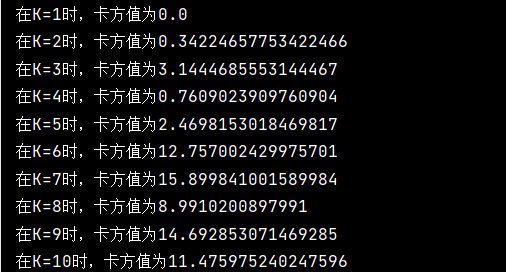
\includegraphics[scale=0.5]{10^5卡方.png}
    \caption{$N=10^5+1$}
\end{figure}

在显著水平$\alpha =0.05$条件下,由卡方分布表可得:
\begin{figure}[H]
    \centering
    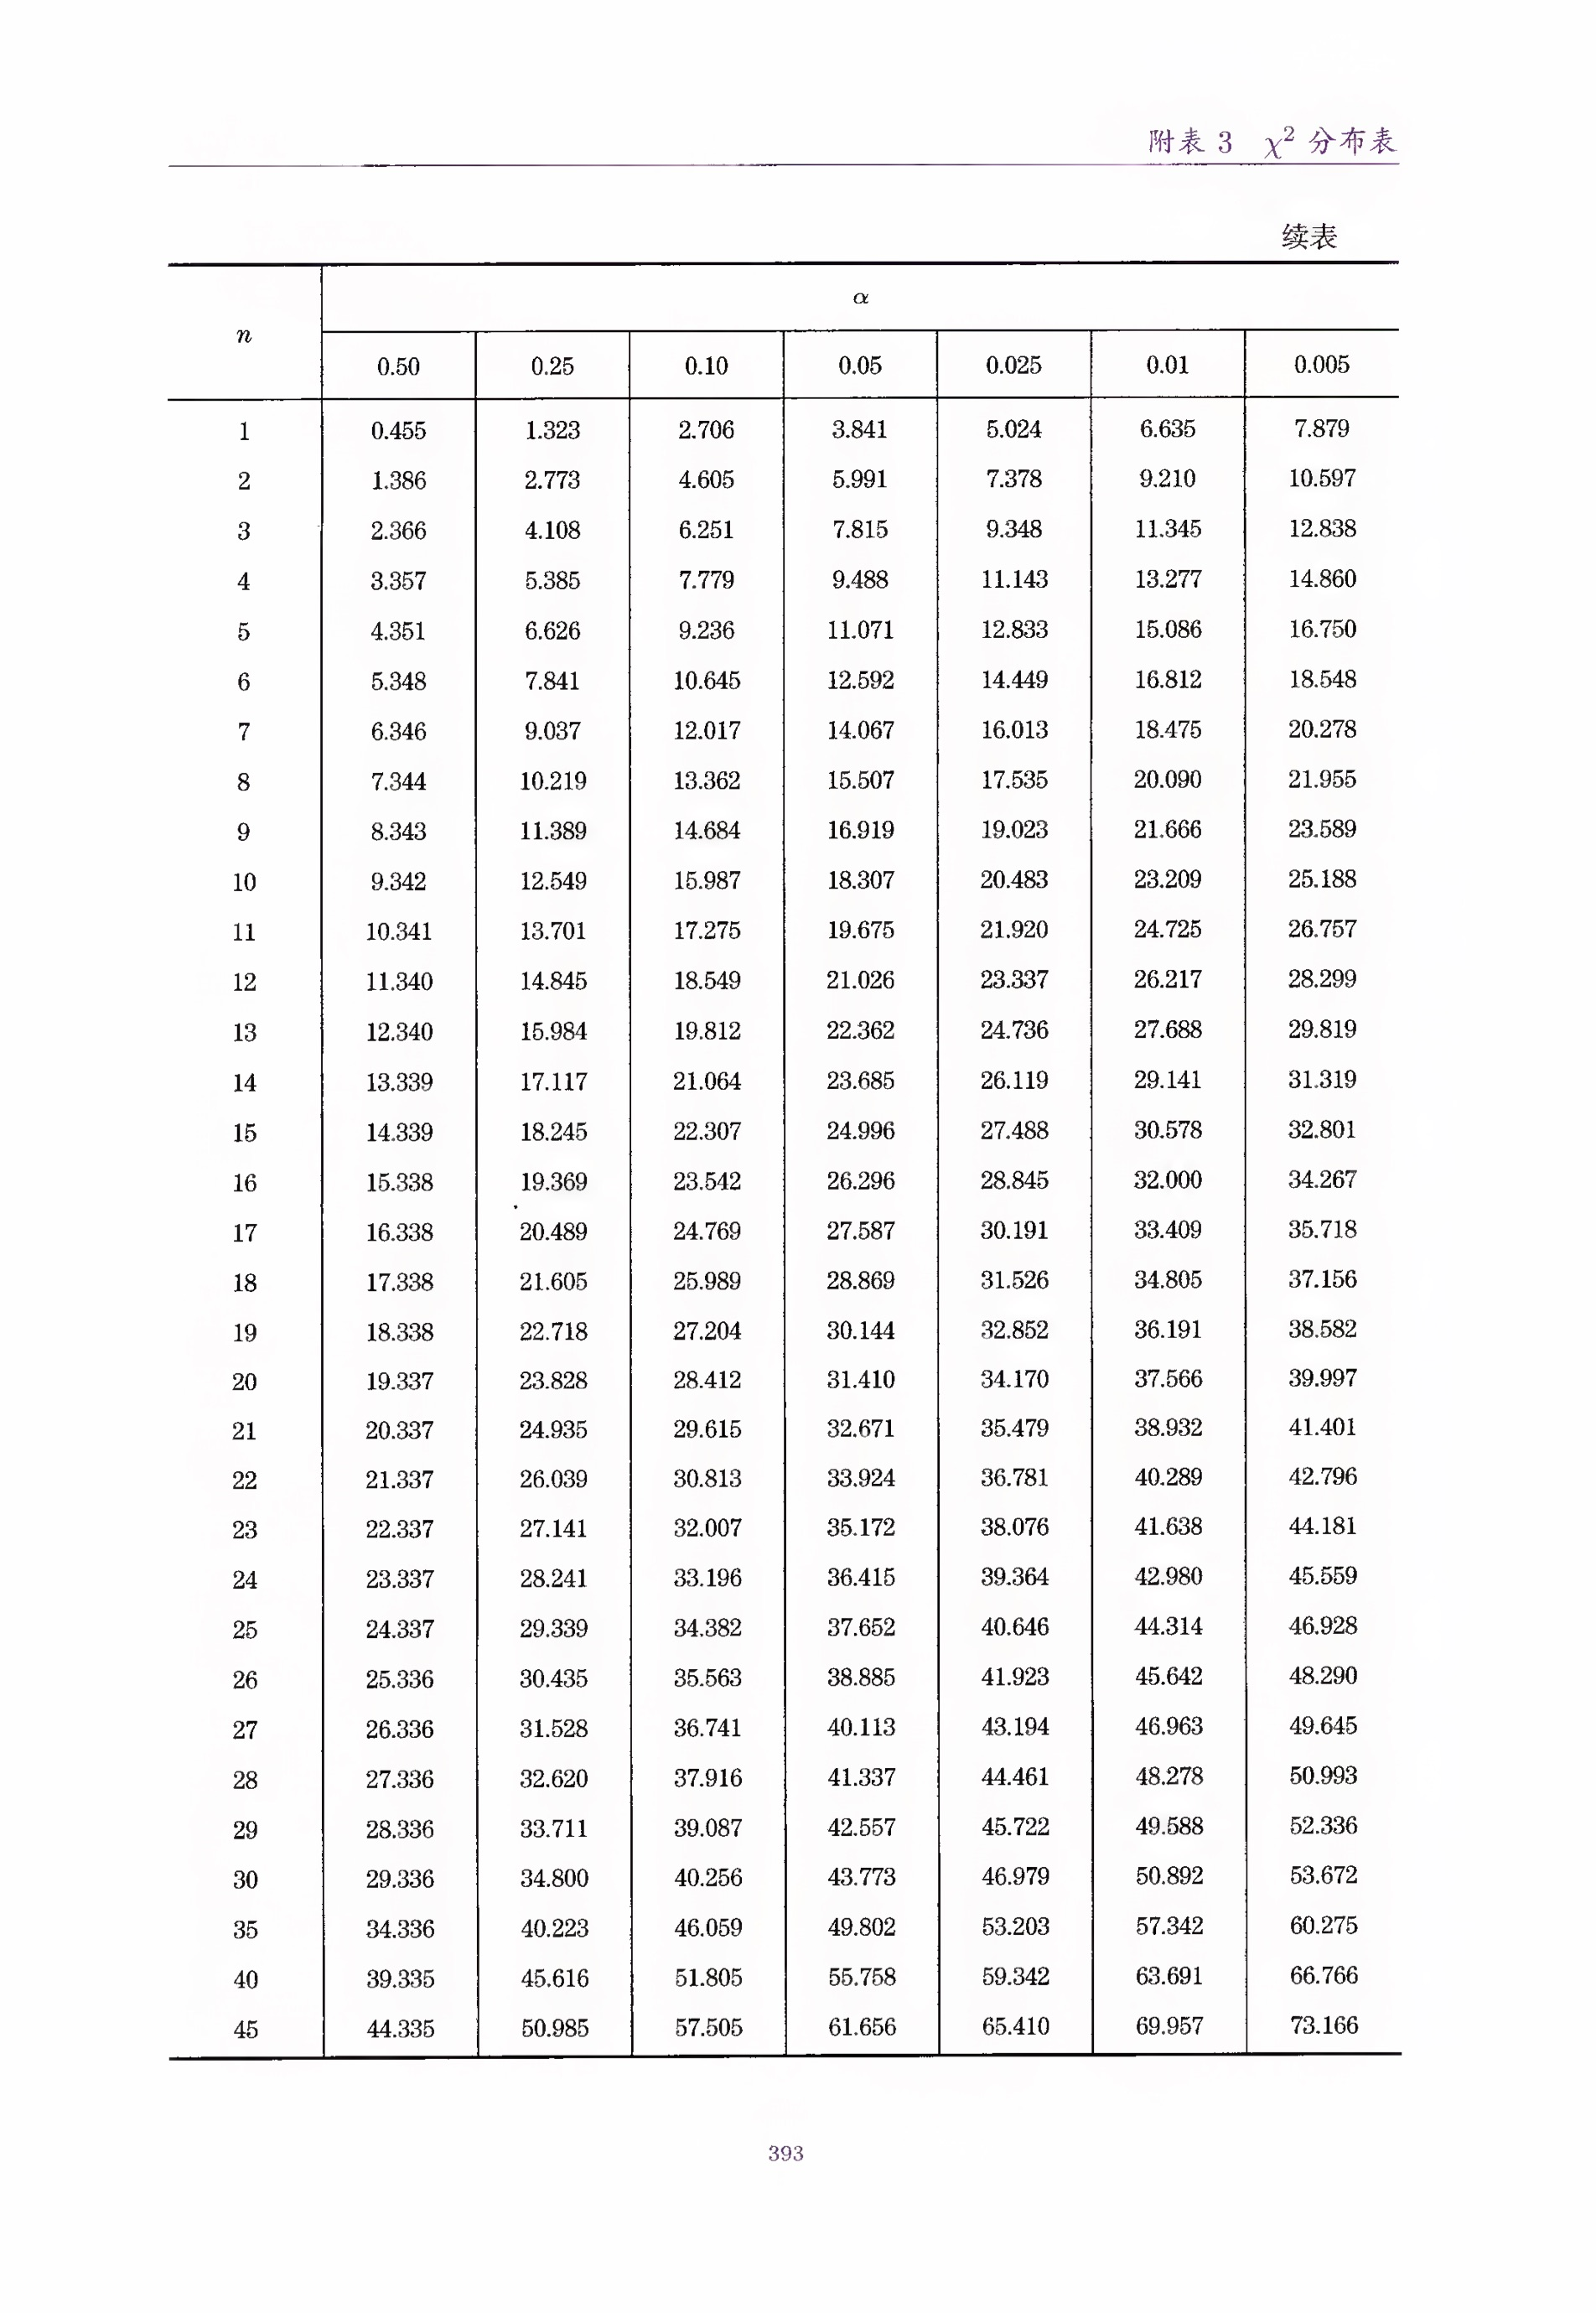
\includegraphics[scale=0.1]{1}
    \caption{卡方分布表}
\end{figure}

$\chi $均小于$\chi _\alpha $,故在置信度$1-\alpha =0.95$下,随机数的均匀性很好

\subsection{二维独立性检验}
用相邻两个随机数
的自相关函数(或相关系数)来标识伪随机数序列的独立性情况,相关系数越小,
独立性越好.
间距为$l$ 的自相关函数是:
\begin{equation}
    C(l)=\frac{<x_nx_{n+l}>-<x_n>^2}{<x_n^2>-<x_n>^2}
\end{equation}
\begin{figure}[H]
    \centering
    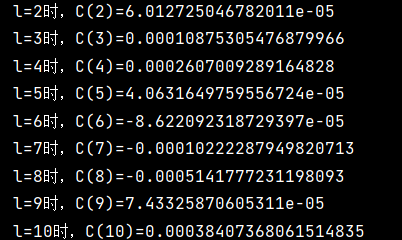
\includegraphics[scale=0.5]{10^7关联.png}
    \caption{$N=10^7+1$}
\end{figure}

可以看出:不同$l$值所对应的$C(l)$值均接近0,故数据独立性很高

\section{总结}
主要学习并掌握了由Schrage方法编写的16807随机数产生程序,以及各种对随机数相关性,均匀性,独立性的检验方法,收获颇多
\end{document}